\documentclass[12pt]{article}
\usepackage[export]{adjustbox}
\usepackage{amsmath}
\usepackage{caption}
\usepackage{subcaption}
\usepackage{times}
\usepackage{graphicx}
\usepackage[left=1in,right=2.5cm,top=2.5cm,bottom=2.5cm]{geometry}
\newcommand{\nd}{\noindent}
\newcommand{\secsize}{\fontsize{15pt}{12pt}\selectfont}
\newcommand{\subsize}{\fontsize{14pt}{12pt}\selectfont}
\begin{document}
\large  
\parskip 3mm 
\tableofcontents
\newpage 
\newpage
\section{\textbf{\secsize{ABSTRACT}}}
This research is aimed at achieving a detailed data analysis and understanding the effect or parameters key to the survival of a person had they been on the ship. Considering the case of Titanic, a British cruise the analysis will be conducted. The survival prediction is done by applying various machine learning algorithms and neural networks. The bio-inspired algorithms will be implemented to optimise the performance of classifiers. Towards the end, accuracies of different algorithms based on features fed to them will be compared in a tabular form.
\newpage
\section{\textbf{\secsize{INTRODUCTION}}}
In the recent industrial era, where science and technology grows exponentially, commercial civilian transportation has turned into a paramount industry. The modes of travel for civilians have never been this elaborate as they are to date. Transportation has become much more standardised and has resulted in greater movement of high density cluster moment. But with this magnanimous scale, there also comes a boon as a result of  fiddling with the laws of nature 

\nd Disruptive effects on transportation systems are cause by anthropogenic disasters which impact infrastructures, terminals and modes. Every from of transport involves nature as a medium of propagation. Air travel involves movement across the vast blue skies and water transportation involves the abundant water masses on our planet. Whenever mankind has shown pride and pretension on its work, nature has always taught it a lesson.

\nd One of the most critical infrastructure in the modern century is defined to be civilian transportation, since a disruption in one of its components can have significant impact on a plethora of lives

\nd Disaster come in two variants : man made or artificial disasters and natural calamities. Natural disasters include floods, volcanic eruptions and earthquakes while man made disasters include terrorism bombings, nuclear leakage and gas poisoining  Certain natural calamities are inherently cause because of man made drudgery which makes this categorization of disasters a conflict in itself . In this essay on disaster management, we will be talking about the importance of disaster management as well as how well countries are prepared for the upcoming disasters.

\newpage

\subsection{\textbf{\subsize{MOTIVATION}}}
\nd To mitigate the risk of disasters in commercial or private civilian transportation, the emphasis on disaster management has never been to this magnanimous scale. Disaster Management plays a paramount role to mitigate the risk during the time of a catastrophe. 

\nd Whenever mankind has shown pride and pretension on its work, nature has always taught it a lesson. On 10th april, 1912, the Rms(Royal Mail Ship) Titanic set sail into the vast atlantic ocean. Titanic was termed as the ”unsinkable” ship. The engineers and architects who designed the vessel were so swollen up on their pride that they skimped many safety measures and deployed less life boats on the titanic as it was, the unsinkable. On the night of 14th april, titanic hit an iceberg in the atlantic and sunk. What was the cost of making an unsinkable ship I ask. 1500 dead including men, women and children. The pride of making an unsinkable ship resulted in one of the most deadliest incidents in the history of civilian transportation and the most extravagant sinking of a superliner or cruise ship to date.

\nd This is the major inspiration for our project. After this incident a majority of the work was focused on risk and disaster mitigation for civilian travel methods. We want to develop and deploy a model, that can help the disaster management authorities to mitigate the risk and increase the probability of surviving of the passengers on board a civilian vessel. Even if our model is able to increase the survival rate incase of a disaster, it will be an honour to have worked on it. Our model predicts the probability of survival of each passenger on board using certain attributes and metrics from a given dataset and this probability can be used by risk and disaster management authorities to facilitate the appropriate amounts of safety precautions on board.

\nd Failures are stepping stones to success even if they are never welcomed. The reasons for failure are often highly unambiguous and highly unconditional.It is a trickster with a sense of cunning and irony which takes pride in tripping people when success is right at the end of the tunnel 

\newpage

\section{\textbf{\secsize{LITERATURE REVIEW}}}
Certain works have been proposed to analyse the data from the titanic, as a result of the incident's unprecedented scale.  Some of the techniques which have been reviewed and executed on the titanic data include a data mining approach to extract cumulative features and highlight higher correlations, using spectral feature selections as a part of scavenging the remains of the ship underneath the atlantic and an approach to normalise the data by using gaussian kernel parameter filtering for implementing on support vector machines. 

\newpage

\subsection{\textbf{\subsize{METHODS USED IN BASE PAPER}}}
Some of the methods used in base paper include the following approaches 

\subsubsection{\textbf{DATA MINING TECHNIQUES}}
 International Journal of Research in Engineering and Technology 2.1, published by Jain, Nikita, and Vishal Srivastava, described the use of data mining approach on the titanic dataset. Analyzing various attributes associated with different types of data, falls under the category of data mining. It is a process of finding patterns and combinations, based upon the fact that the symmetry of the patterns is conserved throughout 

\subsubsection{\textbf{SPECTRAL FEATURE SELECTION}}
In the Proceedings of the 7th International Conference on Software and Information Engineering, Farag, Nadine and Ghada Hassan proposed the use of spectral feature selection for unsupervised and supervised learning. It is one of the techniques used to find relevant features on mixed datasets. For reducing dimensional  hierarchy and for building comprehensible models with highly functional generalization performance, feature selection is used. There are many different feature selection algorithms, which are dependent upon the use case scenario and the heuristics of the problem 

\subsubsection{\textbf{INFLUENCE OF THE SIGMOID FUNCTION PARAMETERS}}
Han, Jun Morag and Claudio proposed the optimisation of the sigmoid function parameters to influence the speed of the convergence of the global cost on the datasets. The high dimensionality of data poses challenges to learning tasks such as the curse of dimensionality. In the presence of many irrelevant features, learning mod-els tend to overfitting and become less comprehensible. For dimensionality reduction and to identify highly coherent features, feauture selection is used 

\subsubsection{\textbf{IMPLEMENTATION OF ID-3 LEARNING ALGORITHM}}
Peng, Wei,  Juhua Chen, and Haiping Zhou proposed the implementation if the id-3 decision tree learning algorithm. ID-3 stands for Iterative Dichotomiser 3, which is a classification approach to solving optimisation problems using the greedy approach. One of the major advvantages of this approach is that it generates understandable prediction rules from the dataset

\subsubsection{\textbf{GAUSSIAN KERNEL PARAMETERS}}
Xiao, Yingchao, et al. proposed the use of gaussian kernel parameters for one support vector machine class and their applications to fault detection. A gaussian is also called as a bell shaped curve, more traditionally, which does an exemplary mode of normalising higher dimensional datasets

\newpage 

\section{\textbf{\secsize{PROBLEM IDENTIFICATION}}}
One of the major challenges that hinders in providing effective disaster management computation is the lack of advanced computers on board commercial vessels. Surely, the current generation of machines demonstrate abilities to compute large chunks of data, but to date, many of the vessels and aircrafts which are being used for transportations are equipped with aged technology because they have been in service since generations. For such vessels and carriers, computing second order partial derivatives of cost functions which are required for traditional gradient descent algorithms will levy a very high computational price. 

\nd In this case we would like to propose the use of bio inspired algorithms. This comes as an analogue to what to teach us survivability better than the nature itself. Bio Inspired algorithms rely on linear algebra based calculations rather than complex higher order partial derivates, like the stochastic gradient descent. This makes bio inspired algorithms much more computationally feasible than standard backpropogation techniques. 

\nd To mitigate the risk of disasters in commercial or private civilian transportation, the emphasis on disaster management has never been to this magnanimous scale. Disaster Management plays a paramount role to mitigate the risk during the time of a catastrophe. 

\nd After the incident of the titanic a majority of the work was focused on risk and disaster mitigation for civilian travel methods. We want to develop and deploy a model, that can help the disaster management authorities to mitigate the risk and increase the probability of surviving of the passengers on board a civilian vessel. Even if our model is able to increase the survival rate incase of a disaster, it will be an honour to have worked on it. Our model predicts the probability of survival of each passenger on board using certain attributes and metrics from a given dataset and this probability can be used by risk and disaster management authorities to facilitate the appropriate amounts of safety precautions on board.

\newpage

\subsection{\textbf{\subsize{OBJECTIVE}}}
The preliminary objective of our proposed model is to predict the probability of survival of a passenger on board a civilian vessel based on various attributes. Our aim is to minimise the risk in the transportation industry and be impactful to help save lives of people. Based on the projections of our model, disaster management authorities can understand which group of people have a lower chance of survival during a catastrophe, and they can implement safety measures in advance to increase the probability of survival 

\nd We also propose using computational methods which rely on linear algebra based calculations which have been derived after observing how the nature survives in the wild. This will not only levy minute computational costs but also boost the run time, lowering it down to exponential values 

\nd We want to develop and deploy a model, that can help the disaster management authorities to mitigate the risk and increase the probability of surviving of the passengers on board a civilian vessel. Even if our model is able to increase the survival rate incase of a disaster, it will be an honour to have worked on it. Our model predicts the probability of survival of each passenger on board using certain attributes and metrics from a given dataset and this probability can be used by risk and disaster management authorities to facilitate the appropriate amounts of safety precautions on board.

\nd One of the emerging algorithms which is based on the principles of biological evolutions and inspired from it, are bio-inspired algorithms, which can be used to develop robust techniques. To address the optimal solutions to complex problems, in the recent years, optimisation algorithms based around nature are being implemented. 

\newpage 
\section{\textbf{\secsize{System Methodology}}}
In our project we have incorporated industry standards of testing and developing the design of our model . We follow some of the universally accepted guidelines for deploying artificial neural networks and machine learning algorithms. These help in easing our flow of work while providing high quality of throughput.

\nd The abstract level steps of the project development are illustrated in the figure below 

\begin{center}
\begin{figure}[h]
\centerline{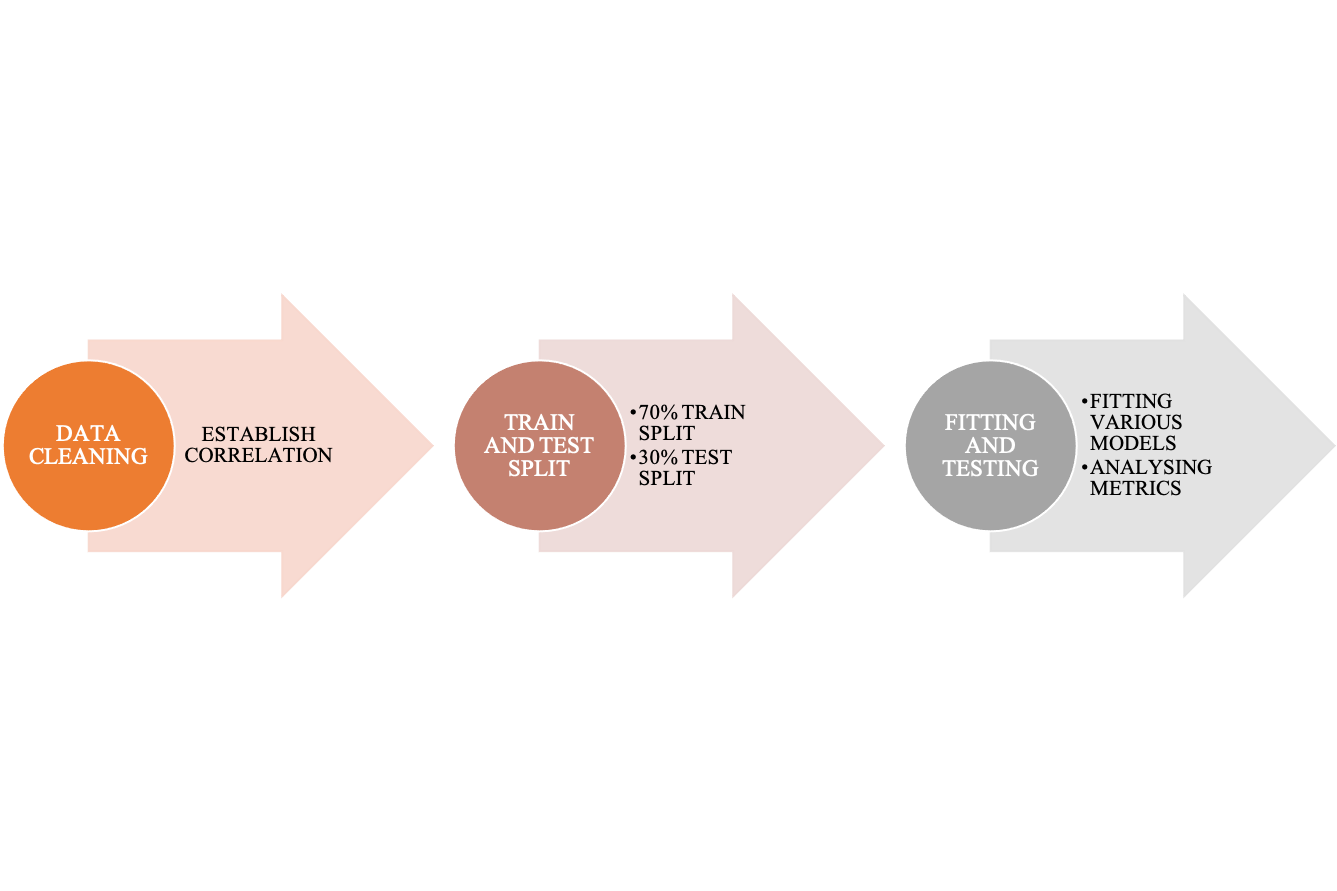
\includegraphics[scale=.6]{flow.png}}
\caption{Process flow chart}
\end{figure}
\end{center}

\nd The broad steps include data manipulation, splitting of the data and testing and fitting of the models. Each of these steps ensure that the consistency in the dataset is maintained and any rogue values are eliminated giving us higher accuracies during the time of testing and training. 

\newpage 

\subsection{\textbf{\subsize{DATA CLEANING}}}
This is one of the major steps which can make or break the entire model. We need to ensure that at every step in the training and testing phase, the model is provided with clean and consistent data. This includes that all the data fed in must be numerical and not categorical, there must be no missing and null values and that strongly correlated attributes are highlighted. 


\begin{center}
\begin{figure}[h]
\centerline{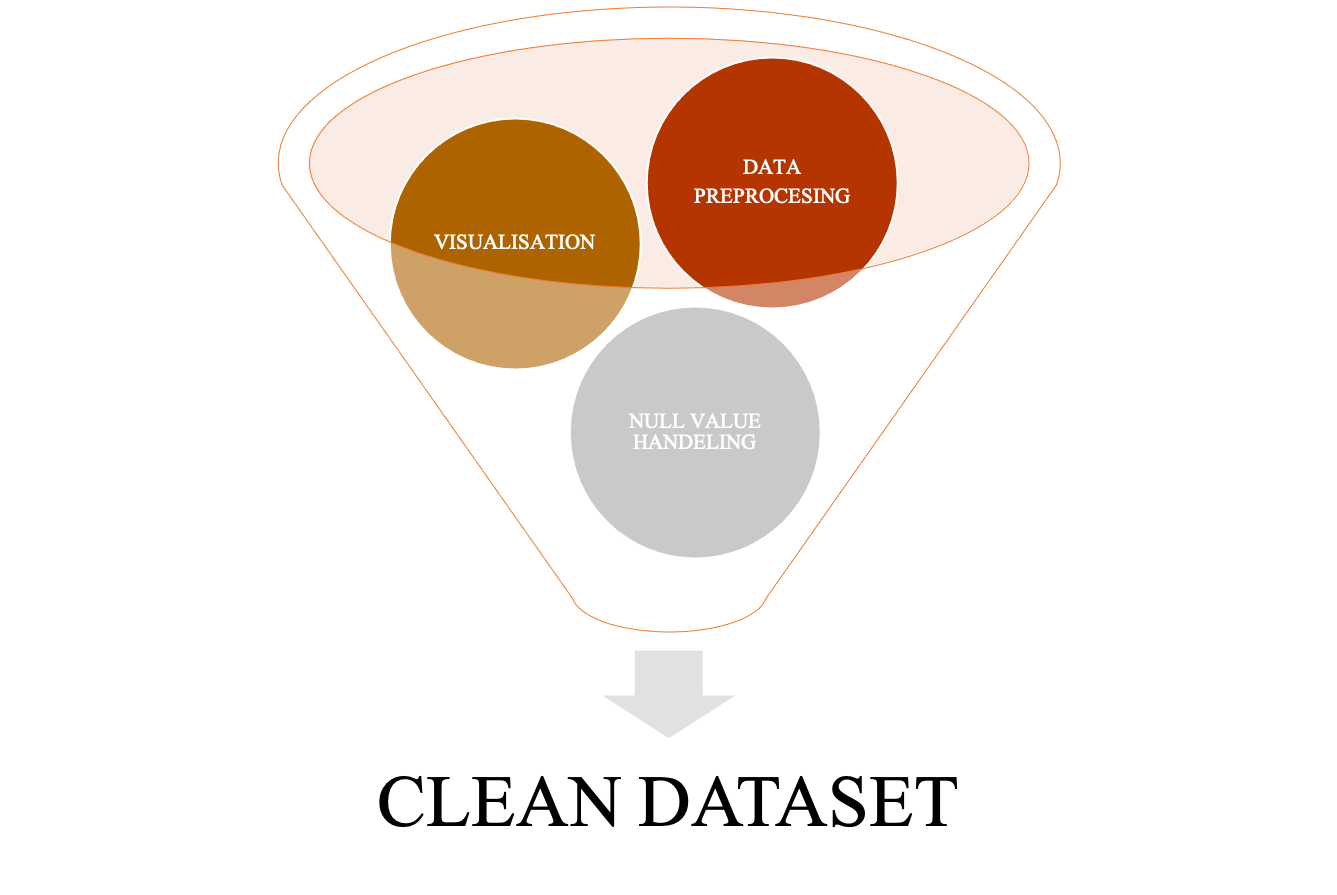
\includegraphics[scale=.55]{datacleaning.png}}
\caption{Eviscerating data }
\end{figure}
\end{center}

\nd All the steps in the data preprocessing phase ensure that the data is highly consistent throughout. Emphasis is largely made on eliminating any occurring null values. The model does not work well under the influence of null values. Having null values increases the chances of bugs and errors in the data model which is highly non trivial. Also this might be highly non trivial, but null values take up more space than other placeholders

\nd All the steps which ensure that there are no null values in our dataset are taken care in the data preprocessing phase. Not only are the null values truncated, but also categorical data must be replaced with equivalent numerical values. This is ensured by truncating categorical data into numeric counter parts. Machine learning models do not recognise categorical data and hence they are truncated. One example of this is changing the label of male and female to 0 and 1 which stand respectively for their mentioned categorical counter parts.

\nd The next part in this process is data visualisation. Knowing before hand, the attributes which are strongly co-related to each other ensures that the model can be emphasised to use them in the appropriate priority. We can setup a priority in training as to train highly co-related values with much emphasis cause these values have a higher chance of boosting accuracy figures 

\begin{center}
\begin{figure}[h]
\centerline{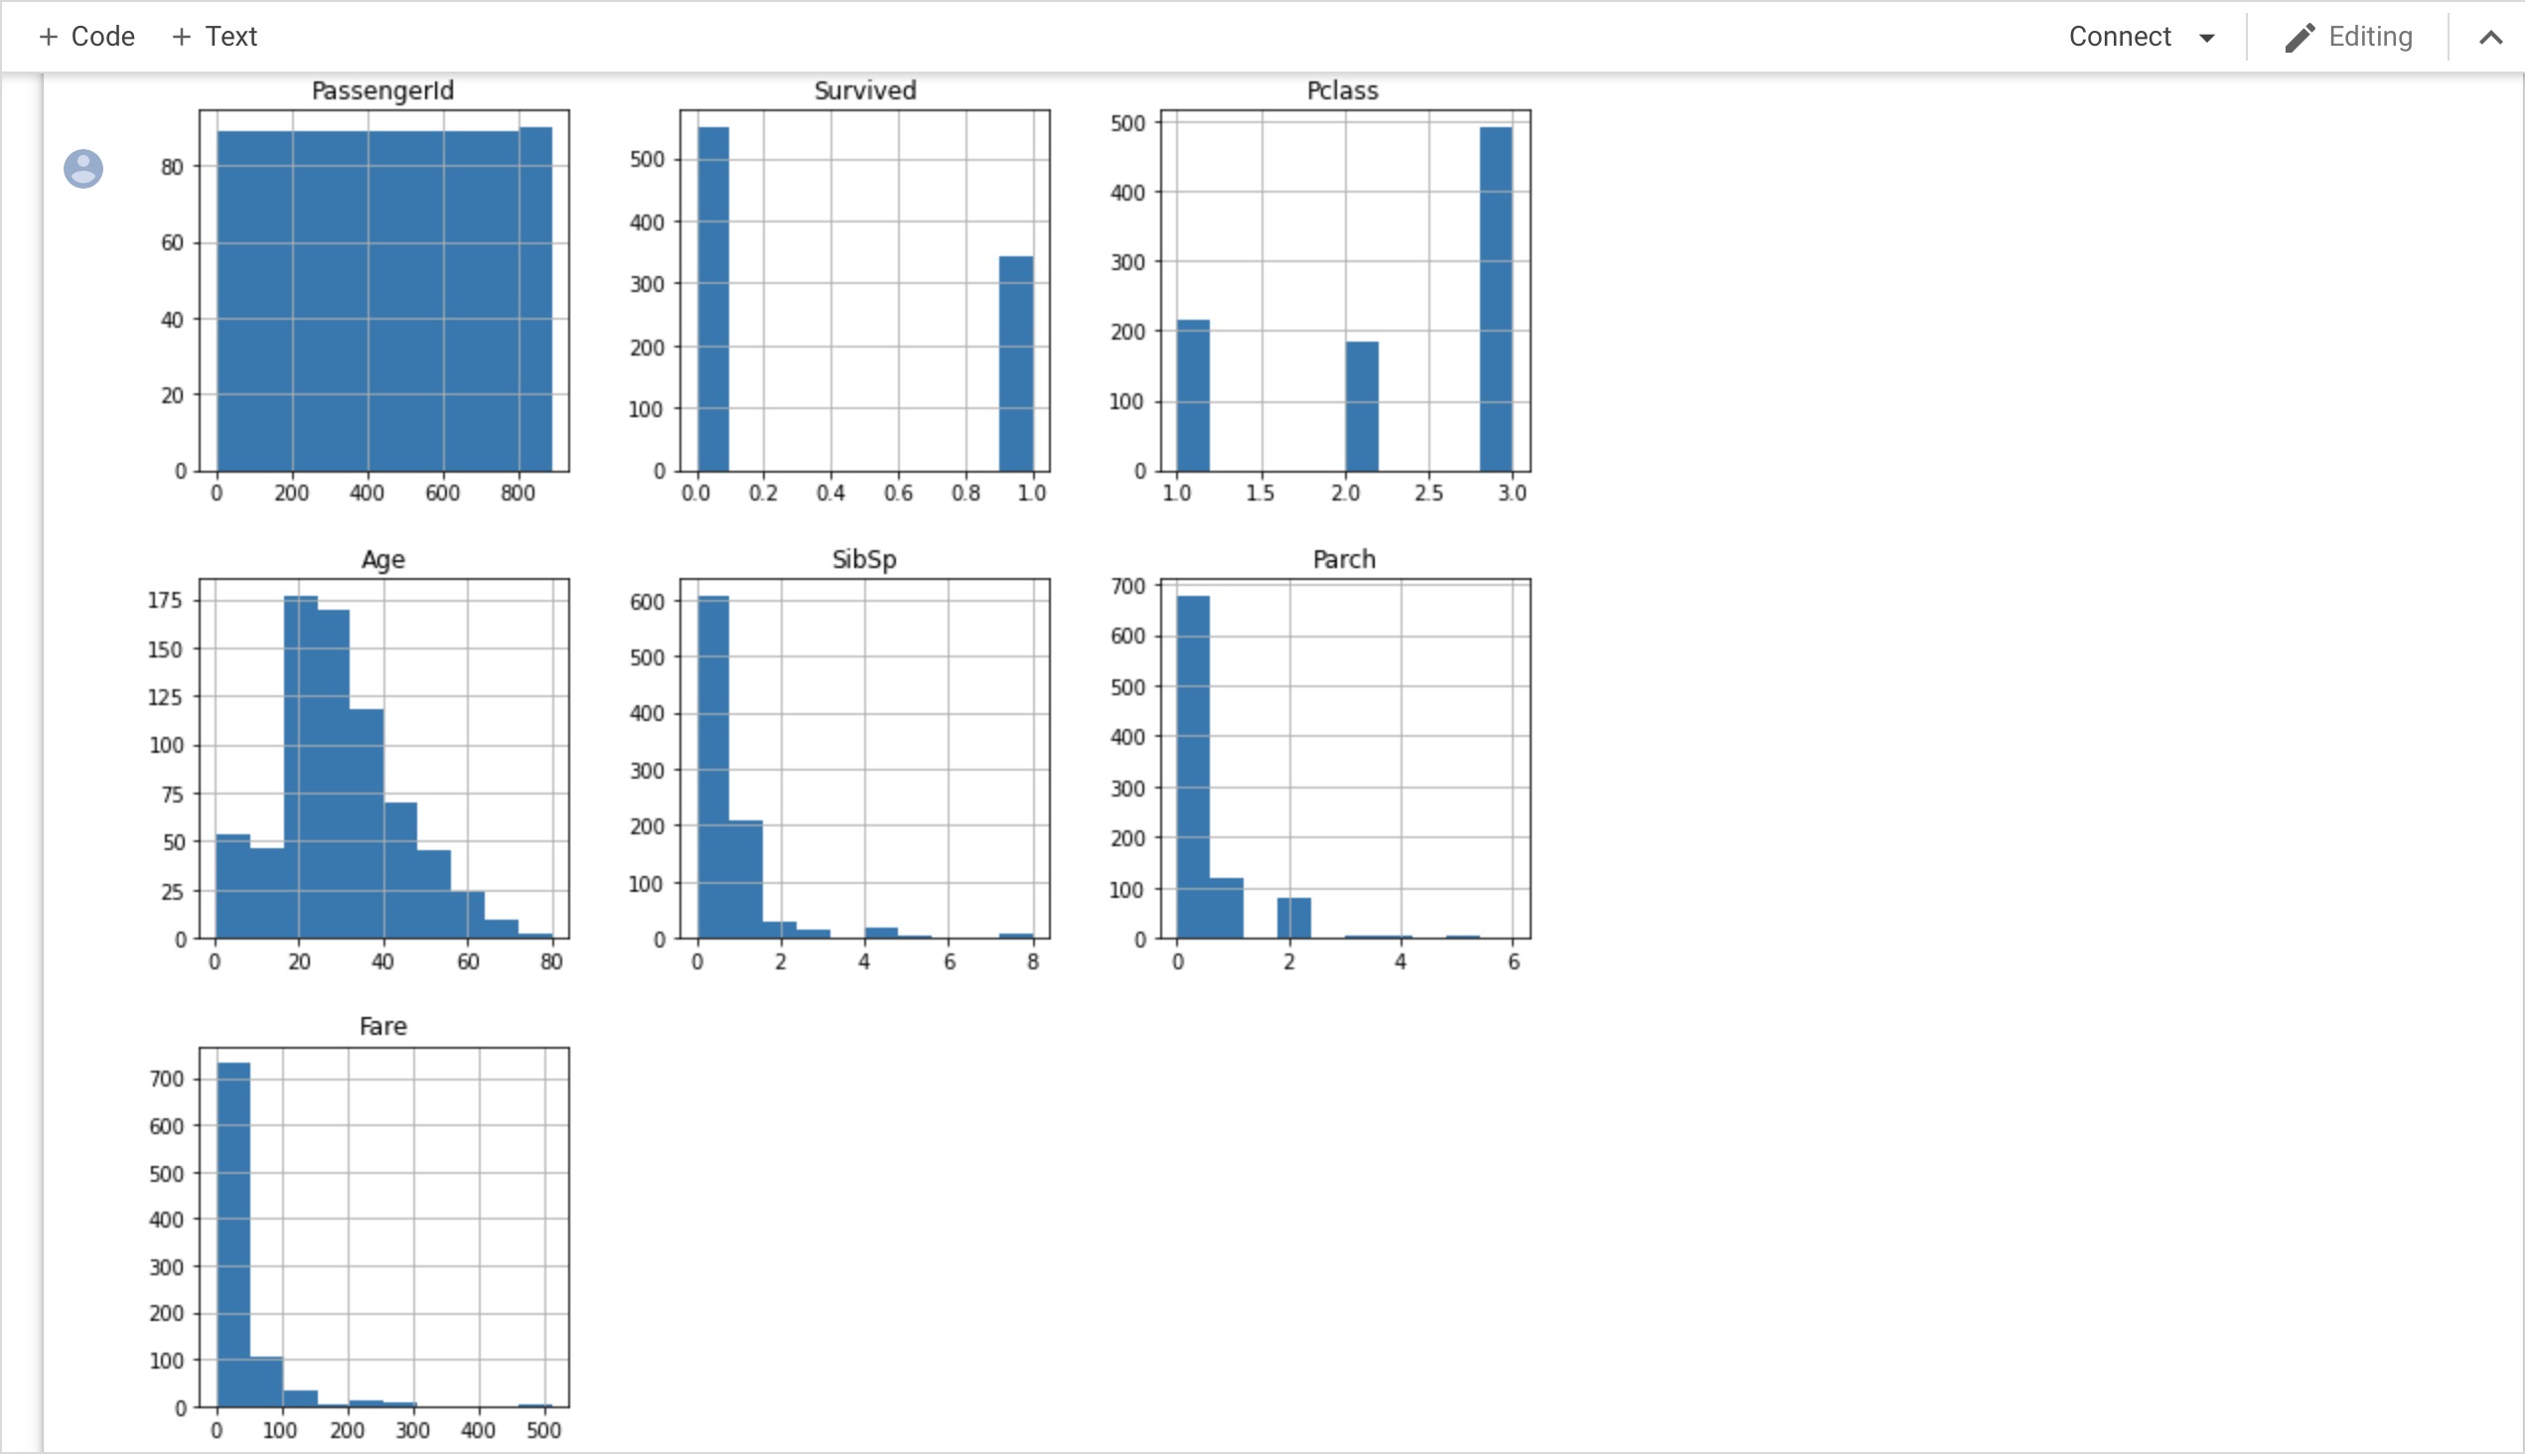
\includegraphics[scale=.32]{visual.png}}
\caption{Data visualising}
\end{figure}
\end{center}

\nd Emphasis on highly co-related data yields a higher chance in boosting accuracy metrics as co-related attributes directly impact on the survivability and probability rates.

\newpage
\subsection{\textbf{\subsize{TRAIN AND TEST SPLIT}}}
We have split the data into 7:3 ratio in which the former part constitutes the training data and the latter the testing data. This ratio is appropriate the provide enough data in the testing phase such that the model neither overfits not does it under fit. This division is a sweet spot for general machine learning algorithms and works like a charm for our proposed as well as base paper implemented algorithms. 

\begin{center}
\begin{figure}[h]
\centerline{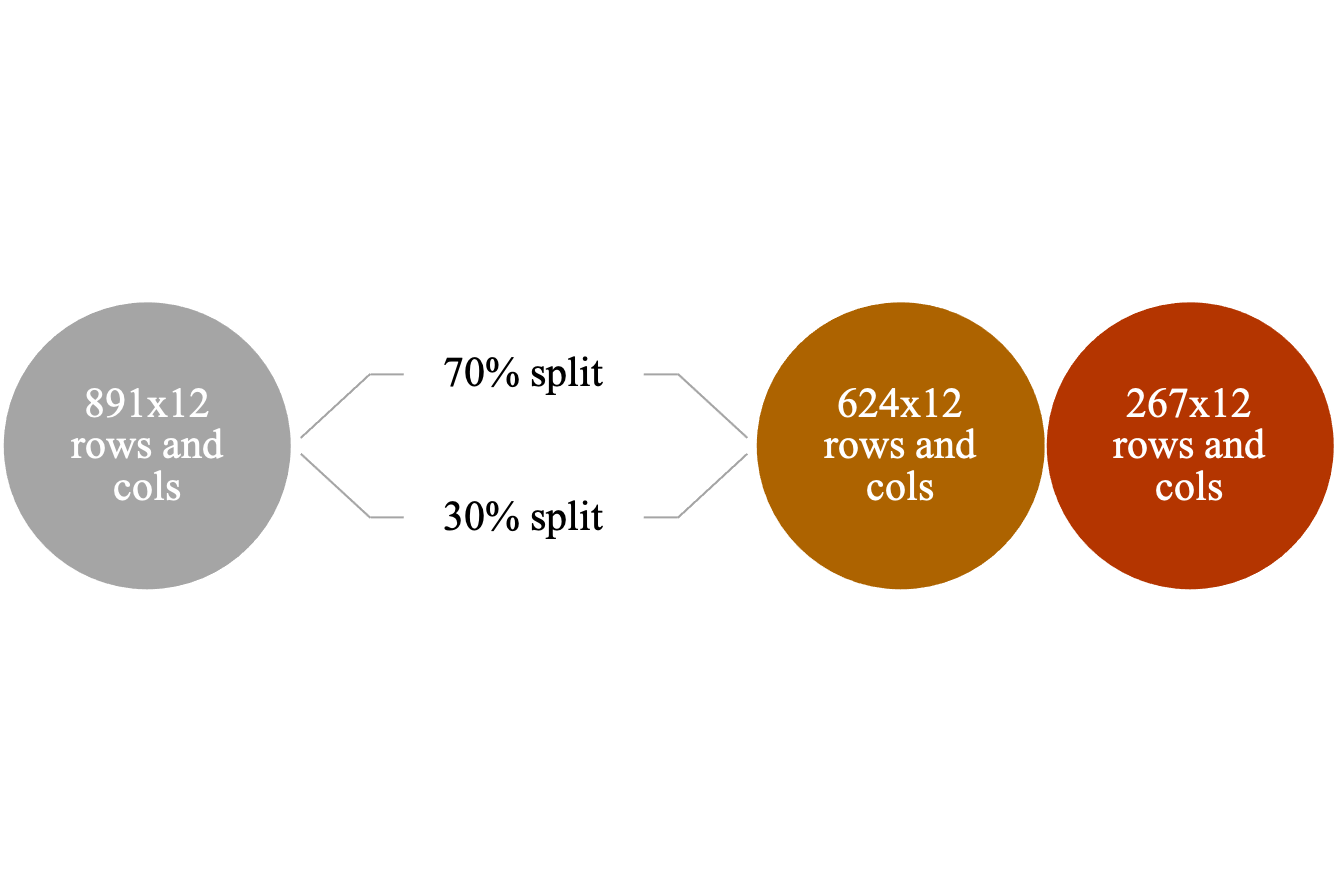
\includegraphics[scale=.55]{split.png}}
\caption{split scale}
\end{figure}
\end{center}

\nd The main dataset contains 891 rows and 12 columns. After performing a 7:3 split the training data consists of the bulk of 624 rows and 12 columns whereas the testing data consists of 267 rows and 12 columns 

\newpage
\subsection{\textbf{\subsize{MODEL FITTING AND TESTING}}}
Now we arrive to the heart of our model, which is the model itself. In this phase we implement both the base paper algorithms which include the machine learning algorithms like support vector machines, decision tree classifiers and such, and also our proposed cutting edge flagship models which are Artificial Neural Networks and Bio-Inspired Particle Swarm Optimisation algorithms. 

\begin{center}
\begin{figure}[h]
\centerline{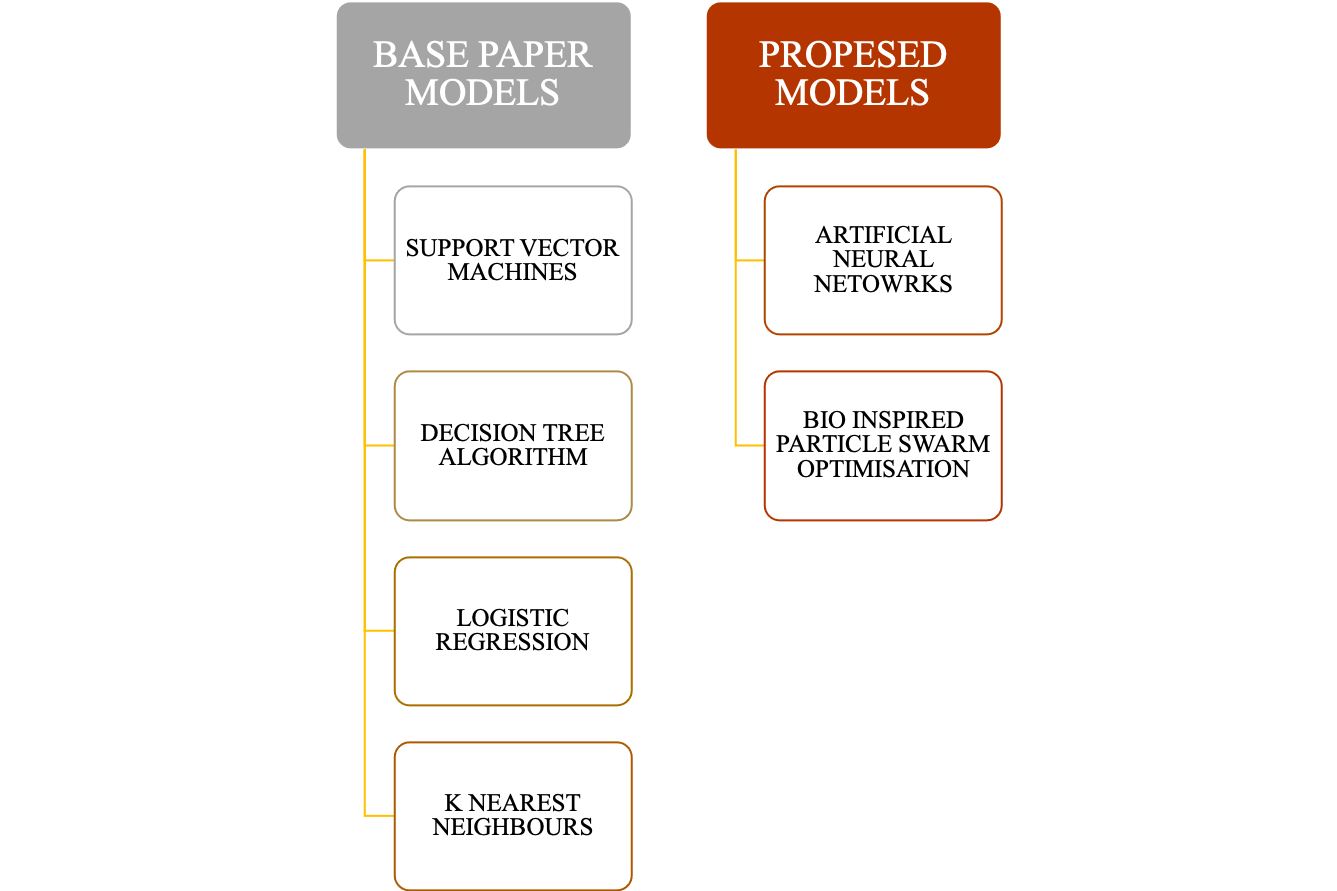
\includegraphics[scale=.75]{models.png}}
\caption{Implemented models}
\end{figure}
\end{center}

\nd These models have been implemented to their highest working accuracy with respect to the dataset and have been observed to output desired results with tremendous accuracies. The accuracies of the base paper model also reconcile with the accuracies mentioned in the paper with corrections upto decimal point margin of errors 

\newpage 
\section{\textbf{\secsize{TECHNOLOGY DESIGN}}}
We have used collaborative, open source and standardised software for building the model. The heart of this model is the Python programming language and the brain of the model is Tensorflow  and Scikit learn libraries. We have ensured that all the technologies used are open source software, as it can be implemented by any disaster management authorities and scaled vertically or horizontally according to their needs without having to pay a penny. 

\nd We have also used data visualisation libraries like Matplotlib and data handling libraries like Pandas. Pandas help to create data frames which are easier to understand by the models and also easy to maintain and handle any future anomalies. Matplotlib functions help us to find highly co-related attributes by providing with methods which can visualise raw data. 

\nd We have also implemented the particle swarm optimisation algorithms from scratch and have built it on top of bio-isnspired code base. With the culmination of these elaborately defined libraries and tools, we were able to create a model could throughput probability survival rates with extremely precise accuracies. 

\nd Scikit learn is written extensively in python itself, and it uses numpy for higher order calculations likelinear algebra and matrix manipulations. It consists of many classes which can be used to implement both supervised and unsupervised machine learning algorithms. 

\nd Tensorflow is a library specifically designed for building complex neural networks. By using tensorflow one can build convolutional neural networks, Recurrent Neural Networks and can train them using different functions and optimisers. Tensorflow is completely open source and is used throughout the industry to build scalable artificial intelligence models. It is based on differential programming, and it treats objects as tensors. A tensor can be thought of as a high dimensional vector in pure mathematics. 


\newpage
\subsection{\textbf{\subsize{ENVIRONEMNT SETUP}}}

\nd Python is the heart of the model. The entire source code as well as the driver code is written strictly in Python programming language. Python is an interpreter based language which is used to for general as well as scientific programming. It is an high level language which has been built on top of the C programming language 

\begin{center}
\begin{figure}[h]
\centerline{
\includegraphics[scale=.75]{python.png}}
\caption{Python Programming Language}
\end{figure}
\end{center}

\nd Python interpreters are supported for global operating systems and are available for mainstream programming language. It also has many open source reference libraries as well as additional plugins to boost run time like CPython. 

\nd Python has revolutionised how programming at an advanced scale can be implemented at such a collaborative level. It global presence and industry standard as well as open source architecture has enabled it to become on of the leading programming languages in the world. 

\nd We have run the python programming language over the google collaboratory notebooks. Using google colab, it becomes exponentially easier for one to work on collaborative project which specifically involve aspects of data science and artificial intelligence. 

\newpage
\nd We write the code on the Jupyter notebooks and run it on a collaborative google colabs platform. Google colab provides the necessary tools so the the jupyter notebooks run 100 times faster than any other collborative environment. This is the main reason if have suited to use google colabs to run our Jupyter notebooks 

\begin{center}
\begin{figure}[h]
\centerline{
\includegraphics[scale=.45]{colab2.png}}
\caption{Google Colab}
\end{figure}
\end{center}
 

\nd It is highly effective to run arbitrary python code through a web server which specifically include methods of artificial intelligence and data science. It also provides a cloud based graphical processing unit capabilities, so that the system is never handicapped of lack of resources
\newpage
\subsection{\textbf{\subsize{LIBRARIES AND DEPENDENCIES}}}
We have used google Tesorflow and Scikit Learn to implement our models. These libraries are rigorously worked out open source libraries which provide highly effective functions to deploy scalable machine learning and artificial intelligence models. 

\nd Scikit learn is written extensively in python itself, and it uses numpy for higher order calculations like linear algebra and matrix manipulations. It consists of many classes which can be used to implement both supervised and unsupervised machine learning algorithms. 
\vspace{10mm}

\begin{figure}[h]
\centering
\begin{minipage}{.5\textwidth}
  \centering
  
\includegraphics[width=.8\linewidth]{tf.png}
  \captionof{figure}{Tensorflow}
  \label{fig:test1}
\end{minipage}%
\begin{minipage}{.5\textwidth}
  \centering
  
\includegraphics[width=.8\linewidth]{sk.png}
  \captionof{figure}{Scikit Learn }
  \label{fig:test2}
\end{minipage}
\end{figure}

\nd Tensorflow is a library specifically designed for building complex neural networks. By using tensorflow one can build convolutional neural networks, Recurrent Neural Networks and can train them using different functions and optimisers. Tensorflow is completely open source and is used throughout the industry to build scalable artificial intelligence models. It is based on differential programming, and it treats objects as tensors. A tensor can be thought of as a high dimensional vector in pure mathematics. 

\nd Using these two libraries as a framework we were able to implement a plethora of machine learning models with extremely high accuracy rates and completely open source in nature. 

\newpage 
\section{\textbf{\secsize{IMPLEMENTATION}}}
The model has been implemented with python as the backbone programming language and also using libraries like Tensorflow, Scikit learn and Matplotlib. These libraries provide us with extensive tools and work environments so that the models can be deployed and run easily. 

\nd Python interpreters are supported for global operating systems and are available for mainstream programming language. It also has many open source reference libraries as well as additional plugins to boost run time like CPython. 

\nd Scikit learn is written extensively in python itself, and it uses numpy for higher order calculations like linear algebra and matrix manipulations. It consists of many classes which can be used to implement both supervised and unsupervised machine learning algorithms. 

\nd Tensorflow is a library specifically designed for building complex neural networks. By using tensorflow one can build convolutional neural networks, Recurrent Neural Networks and can train them using different functions and optimisers. Tensorflow is completely open source and is used throughout the industry to build scalable artificial intelligence models. It is based on differential programming, and it treats objects as tensors. A tensor can be thought of as a high dimensional vector in pure mathematics. 

\nd In our project we have incorporated industry standards of testing and developing the design of our model . We follow some of the universally accepted guidelines for deploying artificial neural networks and machine learning algorithms. These help in easing our flow of work while providing high quality of throughput.

\nd In the following sections we will lay out the details of the code and how their design and testing in the said environments went by. 

\newpage
\subsection{\textbf{\subsize{CODE}}}
Primarily, in the colab notebook, we start by importing our trivial dependencies which have already been rigorously covered in the previous sections of this documentation. 

\begin{center}
\begin{figure}[h]
\centerline{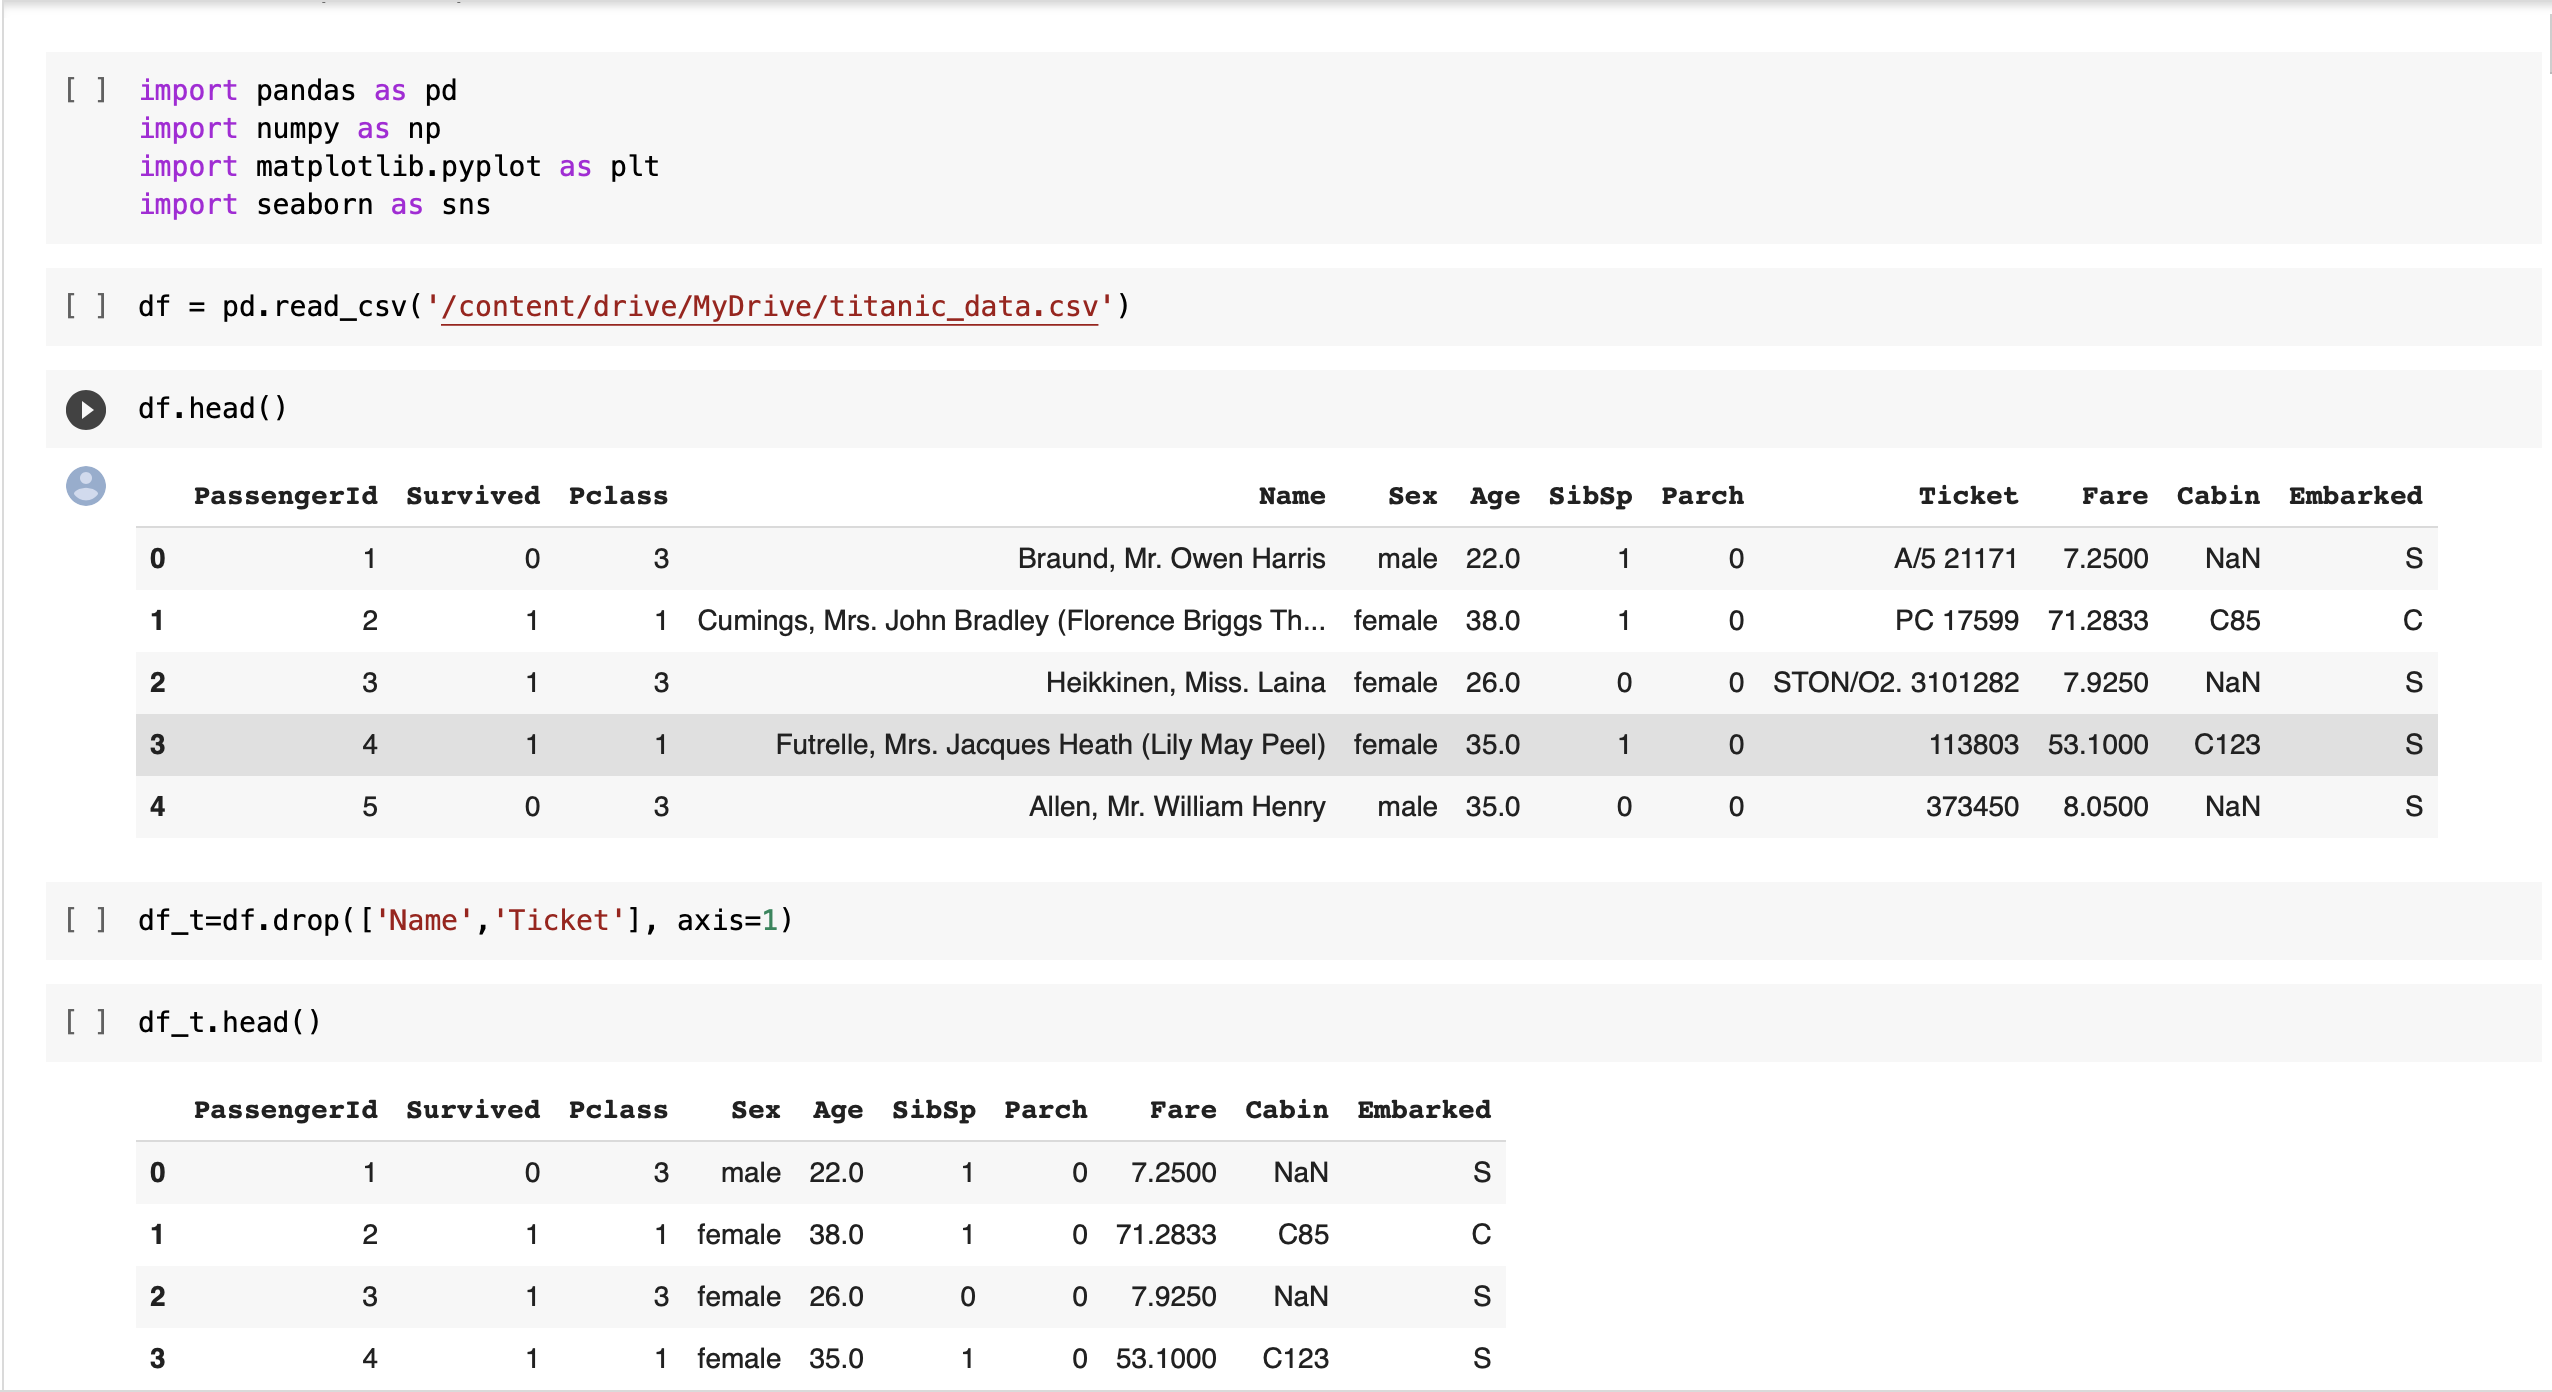
\includegraphics[scale=.35]{part1.png}}
\caption{Importing dependencies and peaking at the dataset}
\end{figure}
\end{center}
 
\nd We import Pandas, for data handling, Matplotlib for visualisation and Numpy for matrix manipulations which will be used in data preprocessing phase. Seaborn is a style of matplotlib which gives certain visual appeal to our graphs and plots. 
\newpage
\subsubsection{\textbf{DATA PREPROCESSING}}
Next we move on to the data visualisation phase. In this phase our aim is to understand which attributes are highly co-related to each other and which attributes correspond the most to improving the accuracy of our model. 

\nd Knowing before hand, the attributes which are strongly co-related to each other ensures that the model can be emphasised to use them in the appropriate priority. We can setup a priority in training as to train highly co-related values with much emphasis cause these values have a higher chance of boosting accuracy figures 
\vspace{10mm}
\hspace{-5mm}
\begin{figure}[h]
\centering
\begin{minipage}{.5\textwidth}
  \centering
  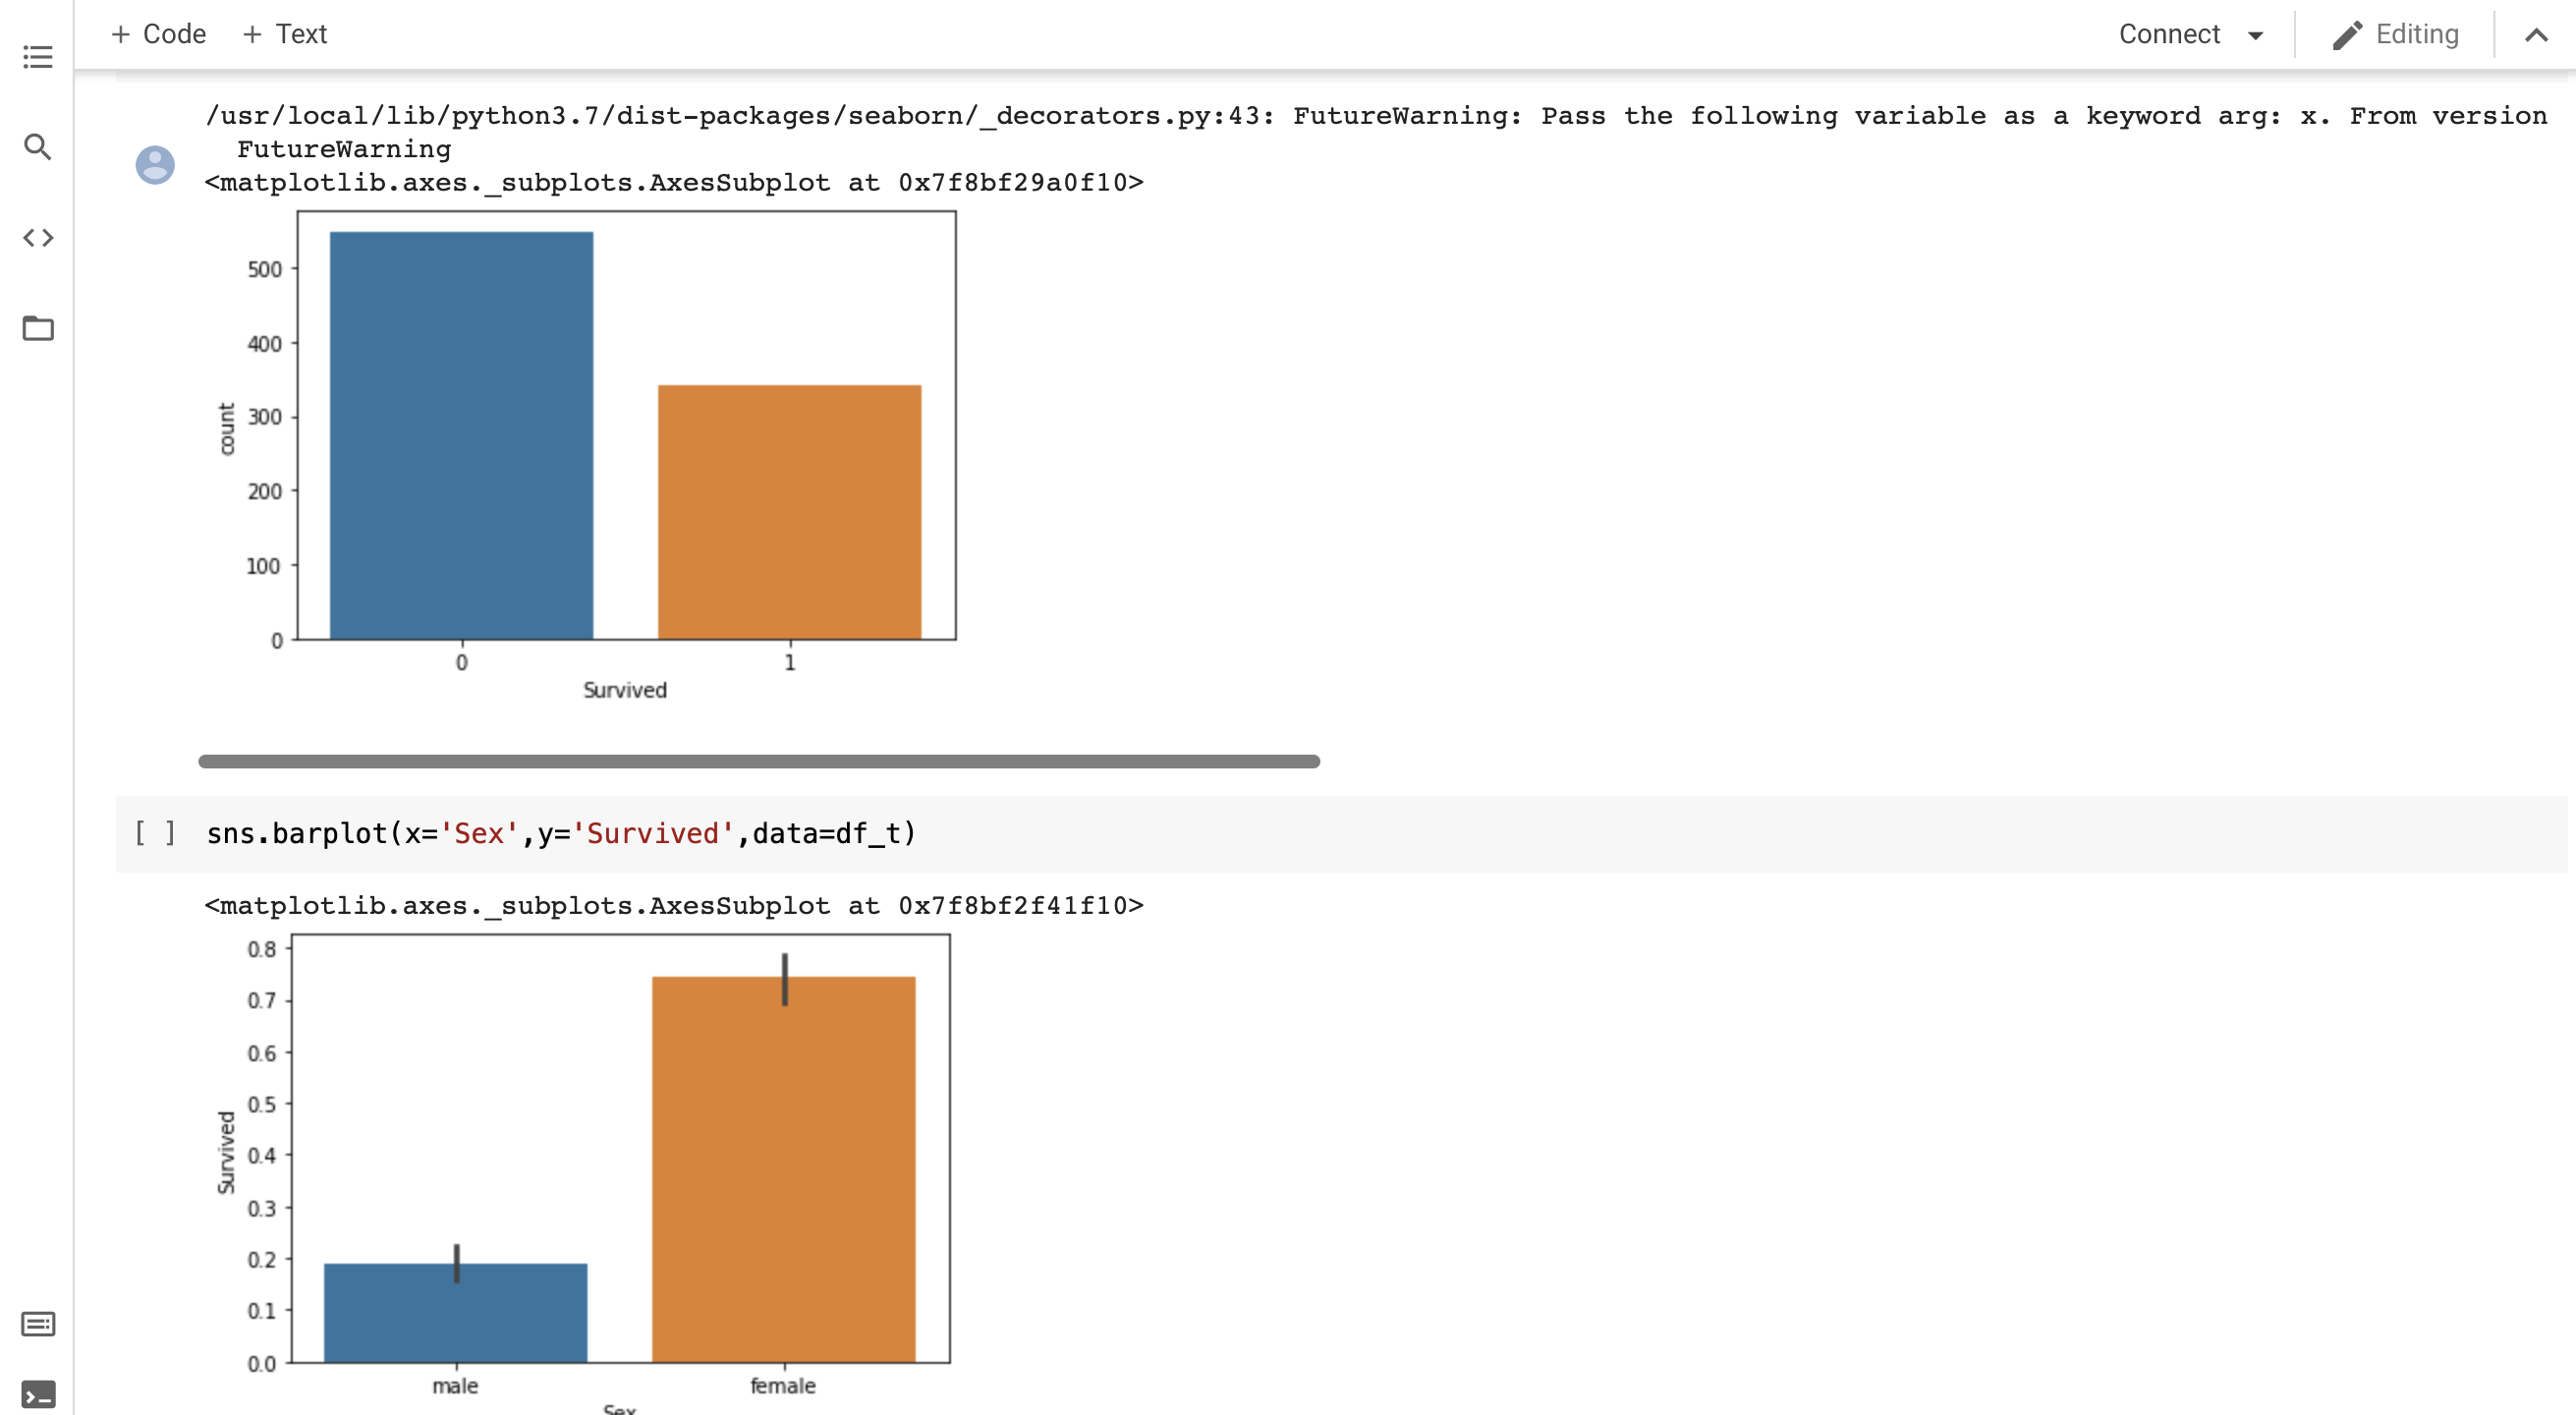
\includegraphics[width=1.2\linewidth]{part3.png}
  \captionof{figure}{Tensorflow}
  \label{fig:test1}
\end{minipage}%
\begin{minipage}{.5\textwidth}
  \centering
  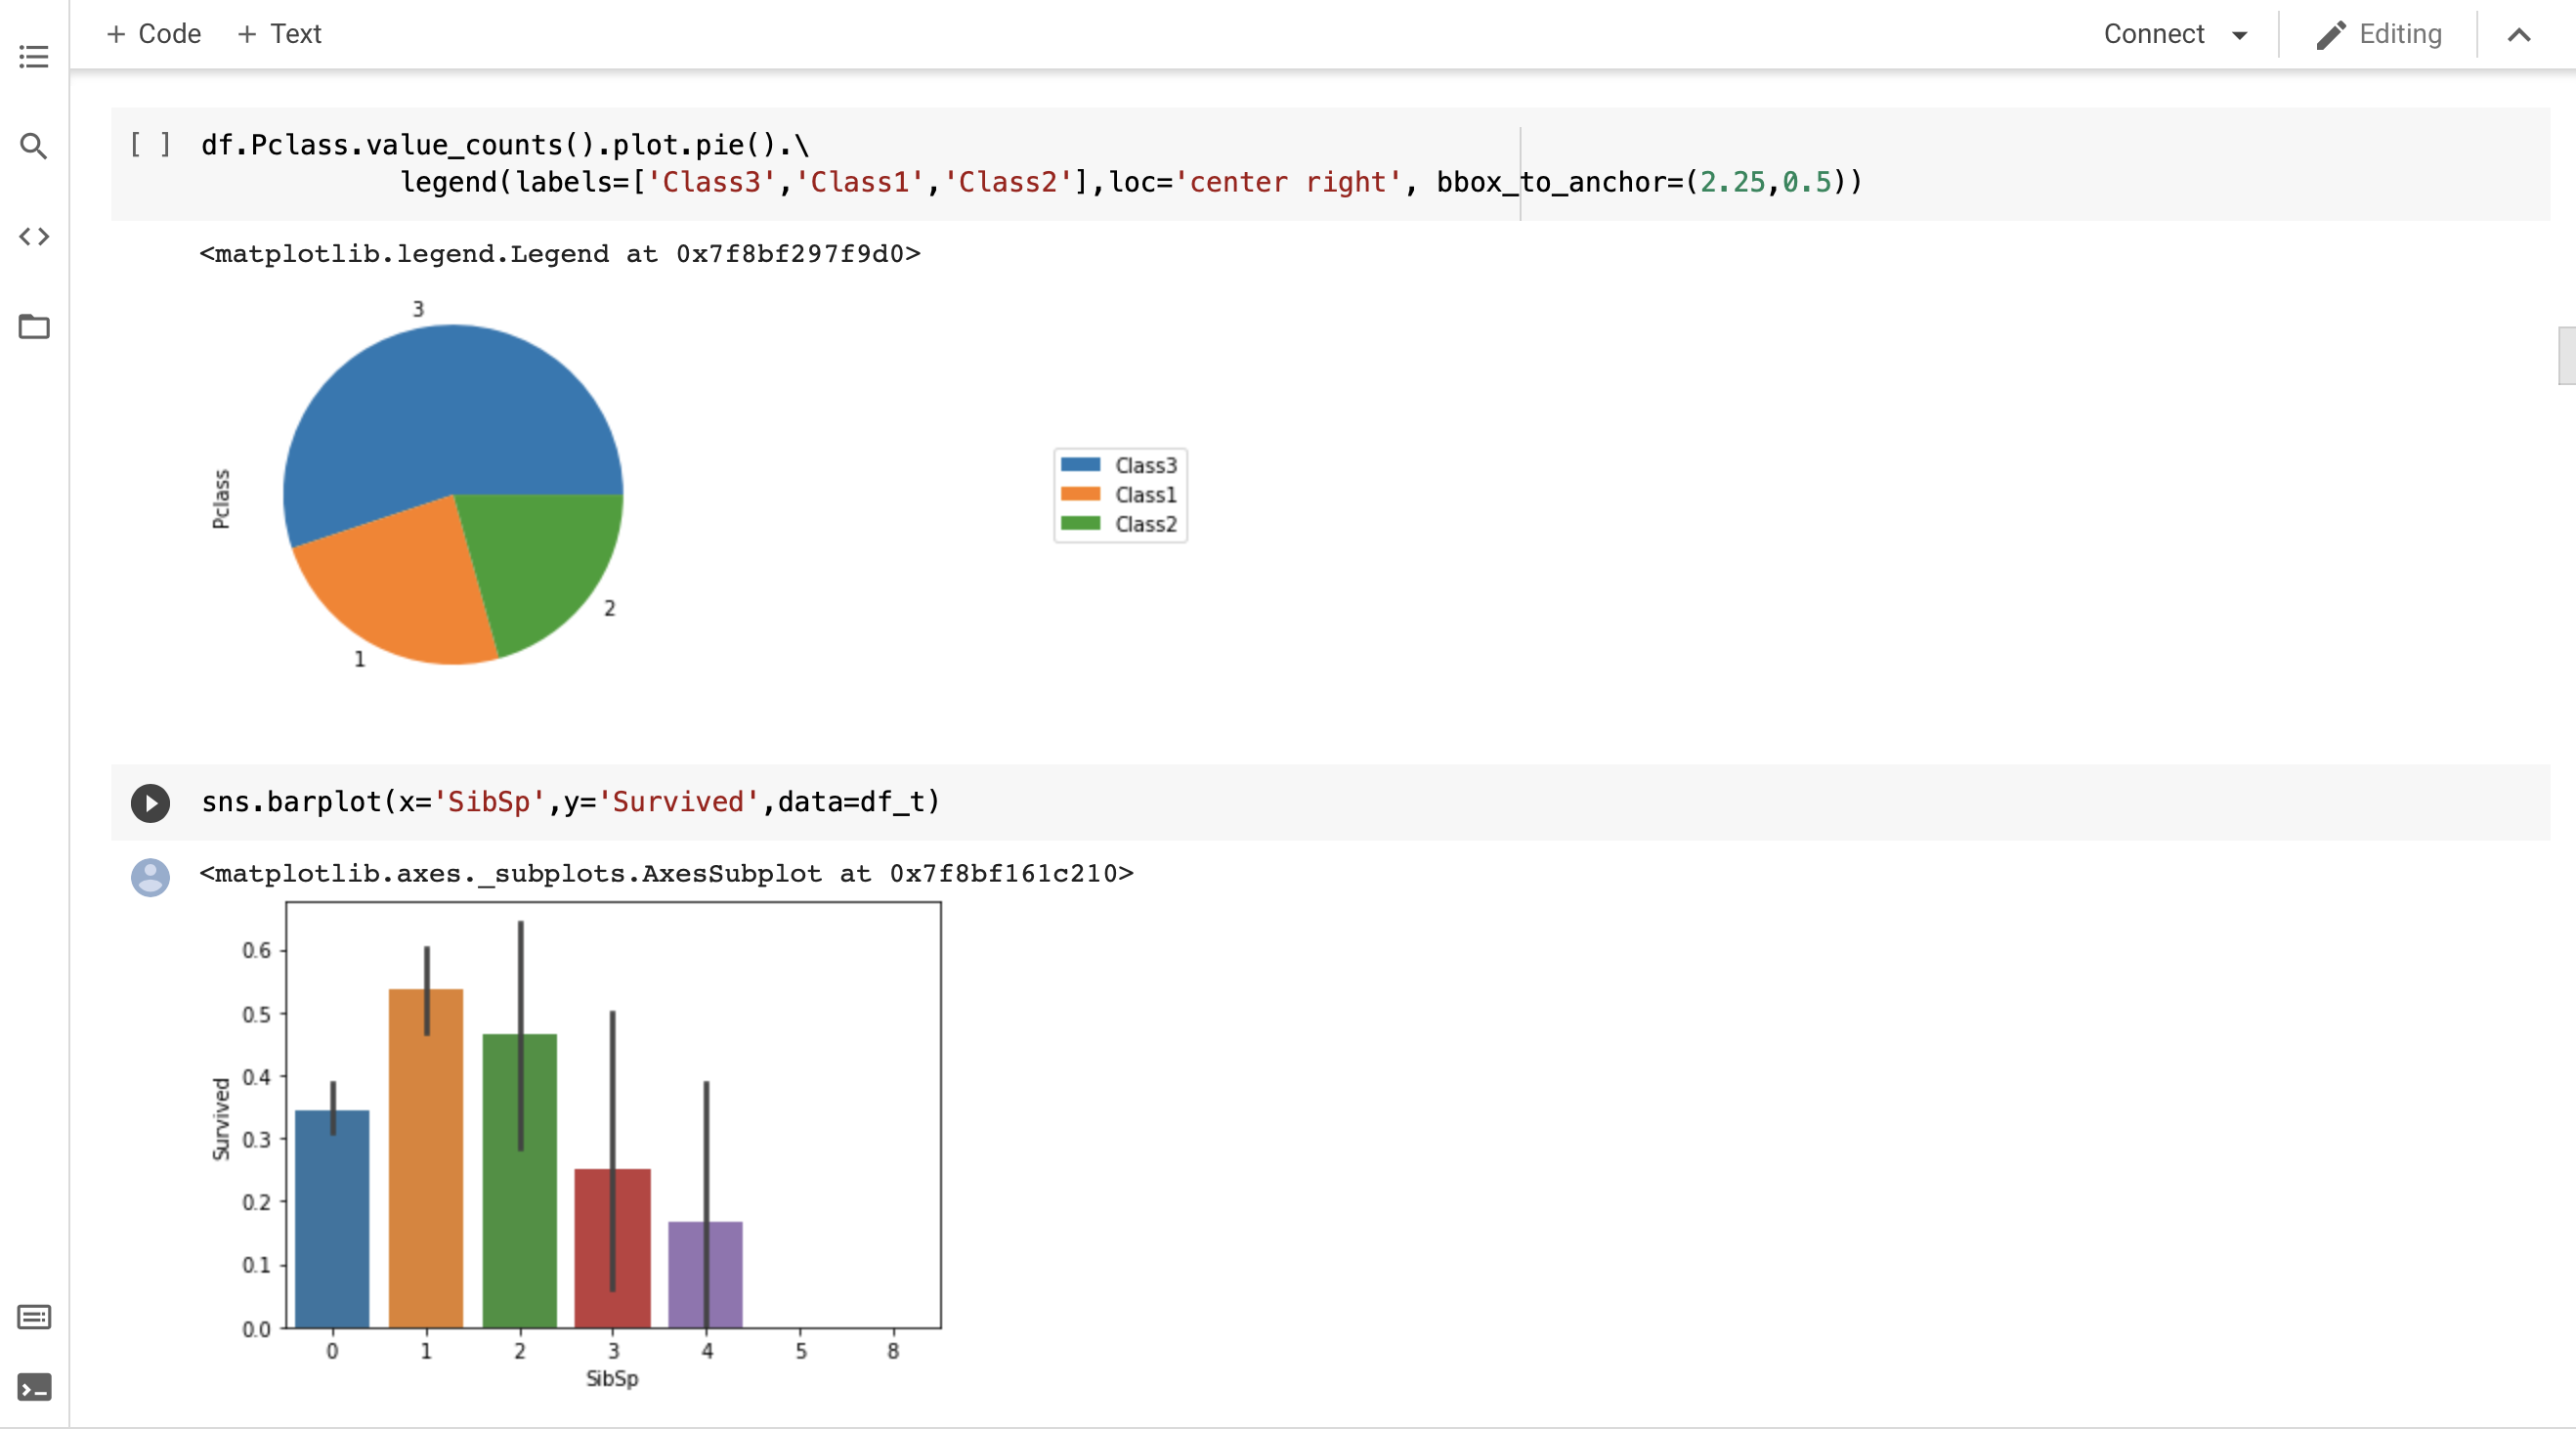
\includegraphics[width=1.2\linewidth]{part4.png}
  \captionof{figure}{Scikit Learn }
  \label{fig:test2}
\end{minipage}
\end{figure}

\nd After getting around the intricacies of the data, we would like to eliminate any null values or categorical data. For this we look at the type of data value each column holds and check for any null values. If there exist any null values, We will truncate those columns

\nd Emphasis on highly co-related data yields a higher chance in boosting accuracy metrics as co-related attributes directly impact on the survivability and probability rates.

\nd All the steps in the data preprocessing phase ensure that the data is highly consistent throughout. Emphasis is largely made on eliminating any occurring null values. Having null values increases the chances of bugs and errors in the data model which is highly non trivial. Also this might be highly non trivial, but null values take up more space than other placeholders

\nd This is one of the major steps which can make or break the entire model. We need to ensure that at every step in the training and testing phase, the model is provided with clean and consistent data. This includes that all the data fed in must be numerical and not categorical, there must be no missing and null values and that strongly correlated attributes are highlighted.

\vspace{10mm}
\hspace{-5mm}
\begin{figure}[h]
\centering
\begin{minipage}{.5\textwidth}
  \centering
  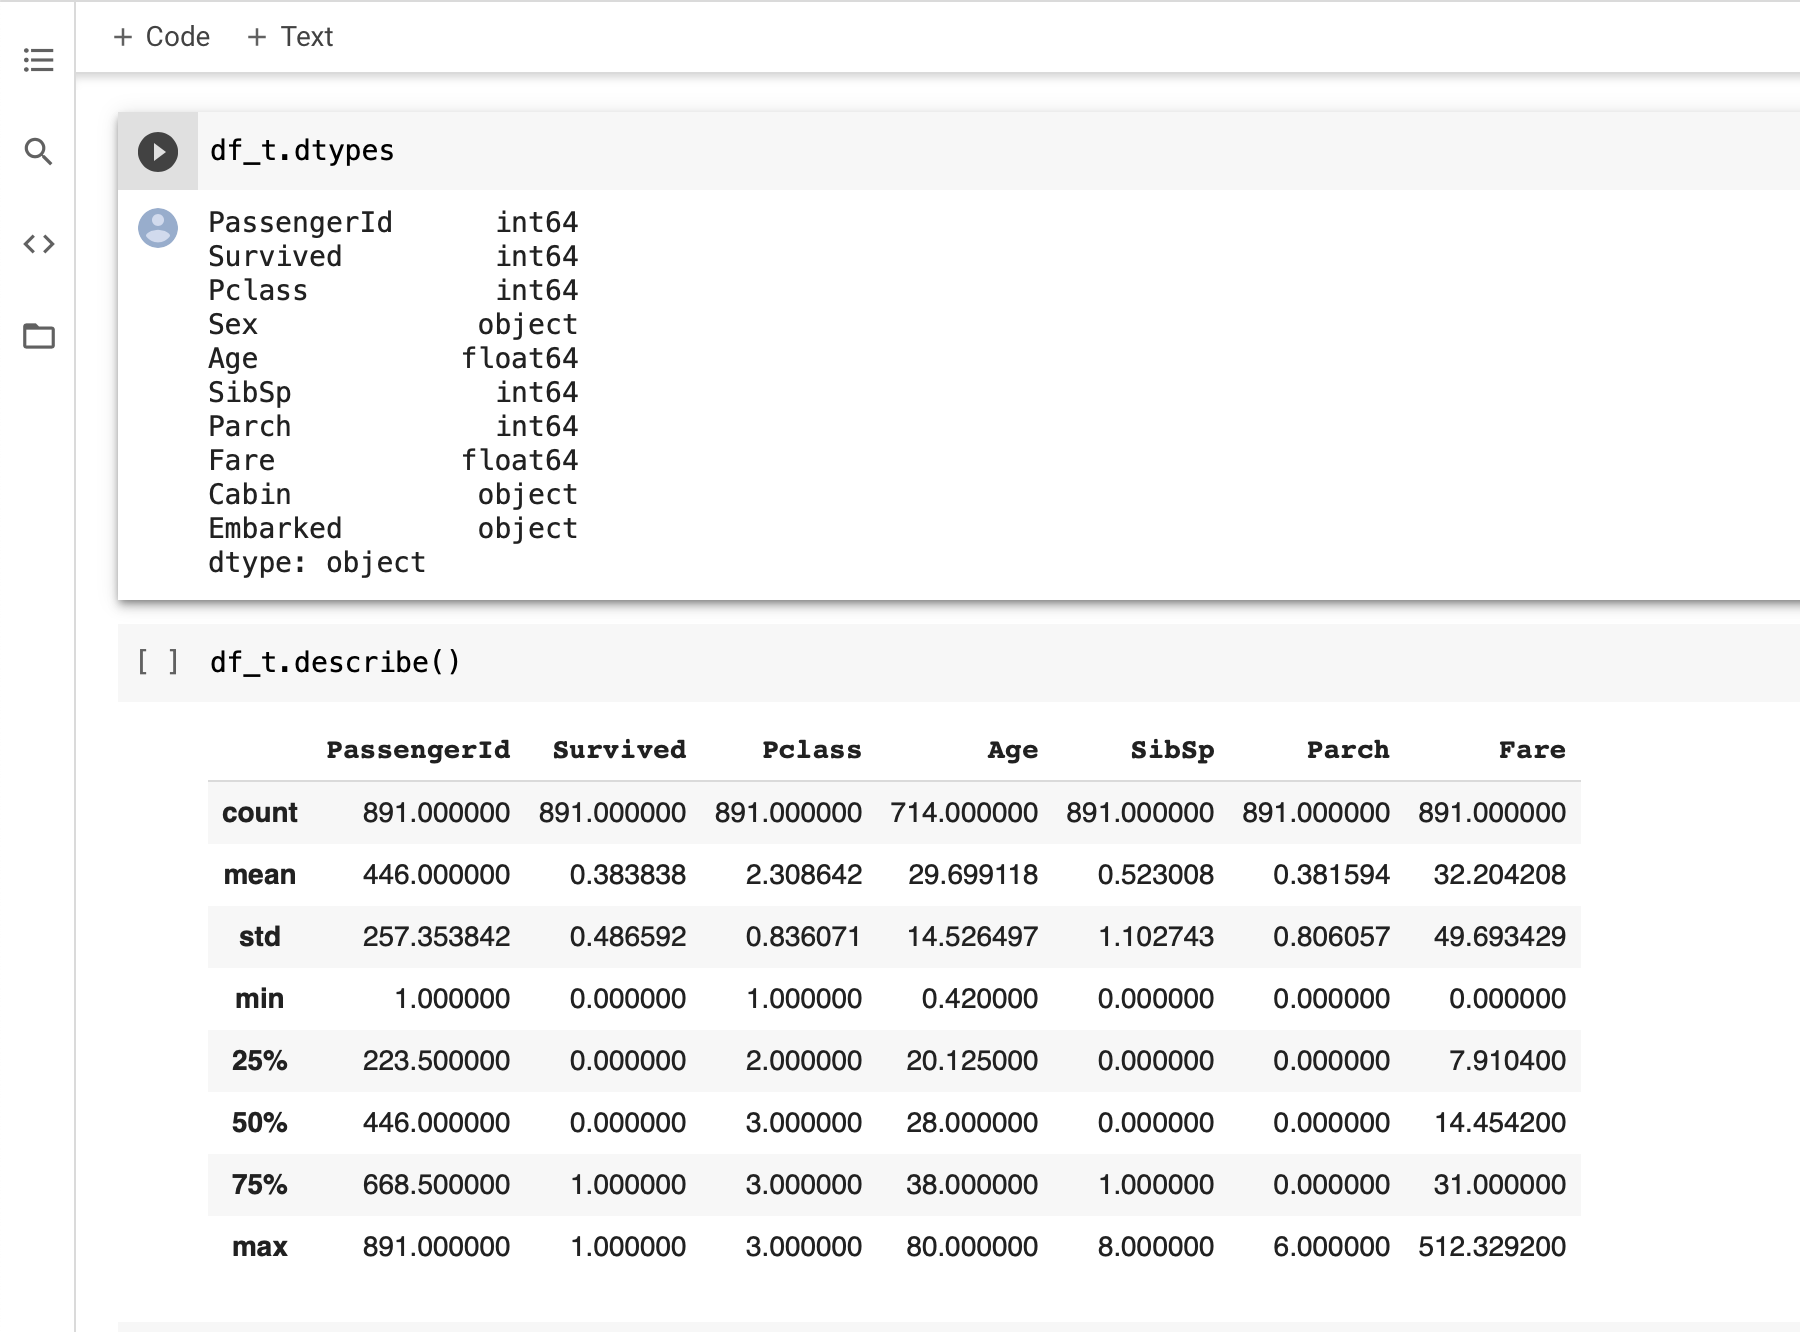
\includegraphics[width=1.2\linewidth]{part5.png}
  \captionof{figure}{Tensorflow}
  \label{fig:test1}
\end{minipage}%
\begin{minipage}{.5\textwidth}
  \centering
  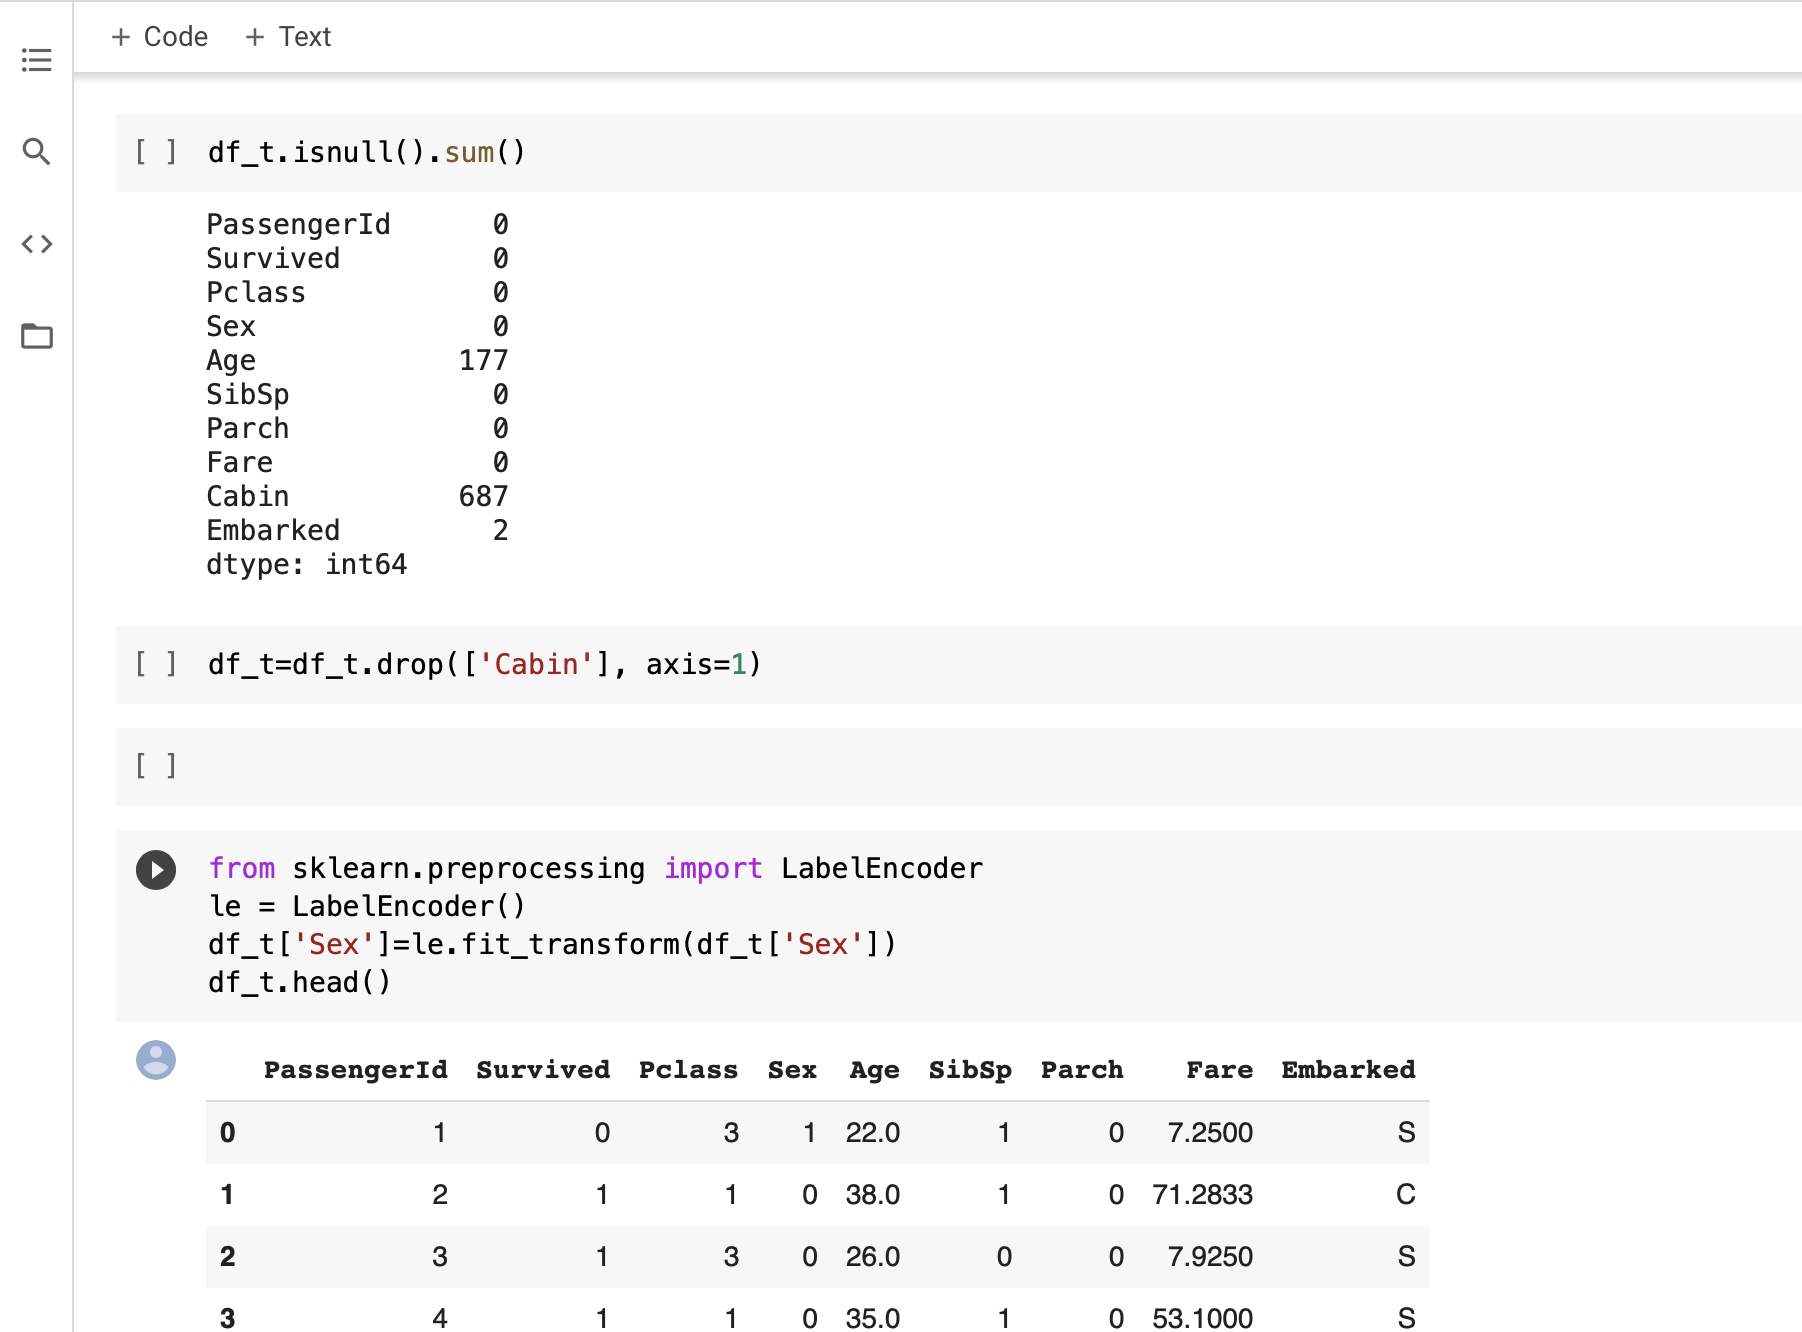
\includegraphics[width=1.2\linewidth]{part6.png}
  \captionof{figure}{Scikit Learn }
  \label{fig:test2}
\end{minipage}
\end{figure}

\nd All the steps which ensure that there are no null values in our dataset are taken care in the data preprocessing phase. Not only are the null values truncated, but also categorical data must be replaced with equivalent numerical values. This is ensured by truncating categorical data into numeric counter parts. Machine learning models do not recognise categorical data and hence they are truncated.
\newpage 
\nd After this step we can see that put data has no null values and that it is highly consistent with no categorical attributes too 

\begin{center}
\begin{figure}[h]
\centerline{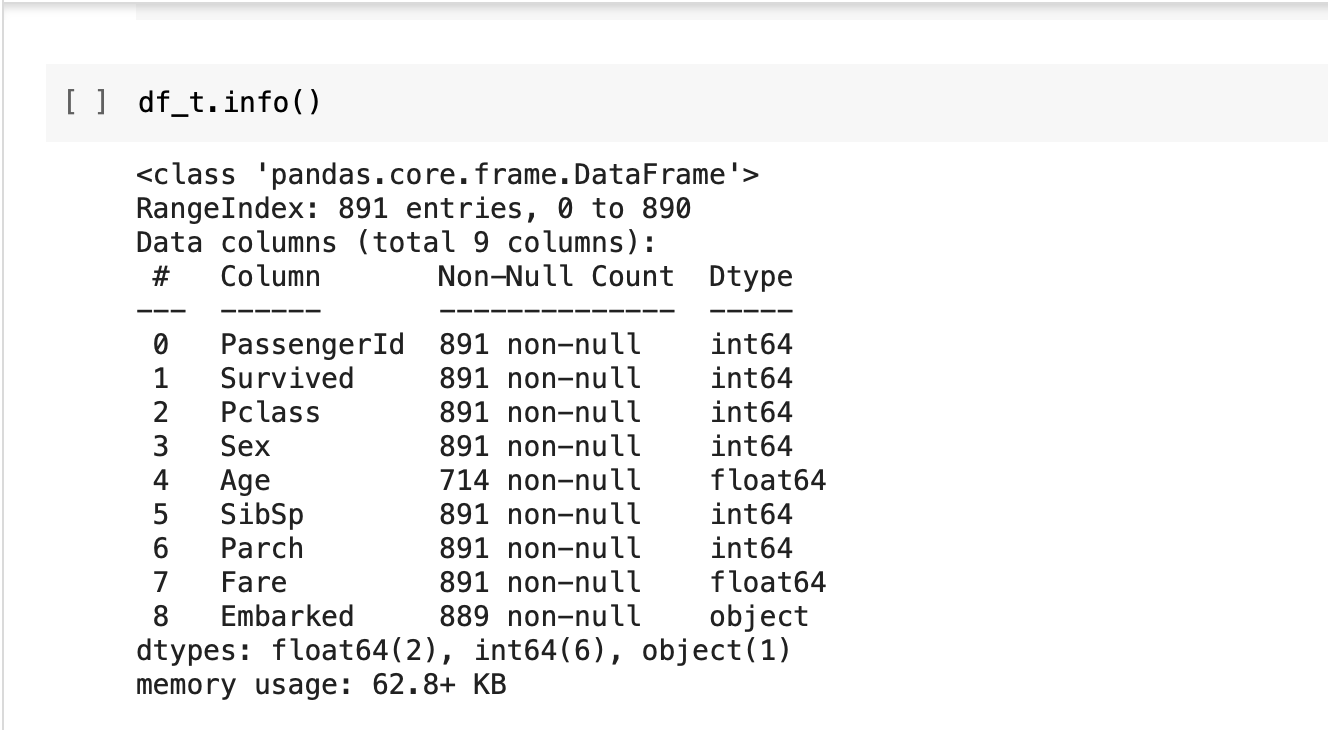
\includegraphics[scale=.35]{part7.png}}
\caption{Importing dependencies and peaking at the dataset}
\end{figure}
\end{center}

\nd We have now successfully truncated all the null and categorical data from our dataset and now we can ensure that our model will be fed with clean and consistent data throughout the entire phase of testing and training. This makes our data highly trivial and ensures consistent accuracies throughout the board 
\newpage
\subsubsection{\textbf{BUILDING THE MODELS}}
Now we come to the heart of our project that is to build the models. We start by exporting all our dependencies and also the library Functions. We implement all the algorithms mentioned in the base paper in a sequential order. 

\nd First we perform our train and test split in the ration of 70 and 30 percents respectively. For this we mention the test size in the code as 0.3 and the remaining 0.7 will automatically be reserved for training 

\begin{center}
\begin{figure}[h]
\centerline{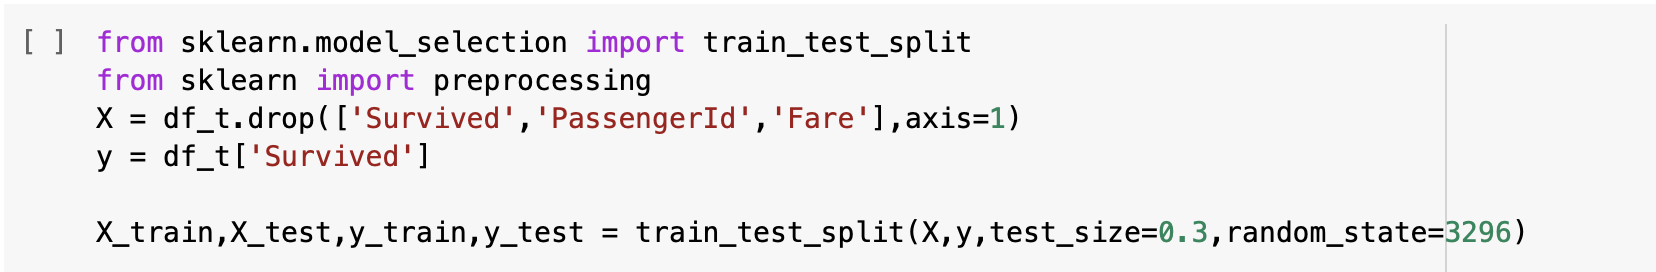
\includegraphics[scale=.35]{1.png}
\caption{Importing dependencies and peaking at the dataset}
\end{figure}
\end{center}


\end{document}